\chapter{Pastes and Modeling Materials} \index{Modeling}

\begin{multicols}{2}

\section{Papier M\^{a}ch\'{e}} \index{Papier M\^{a}ch\'{e}}
\label{sec:paper-mache}

\begin{center}
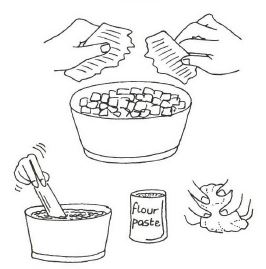
\includegraphics[width=0.4\textwidth]{./img/vso/papier-mache.jpg}
\end{center}

\begin{itemize}
\item Soak pieces of paper or card in
water for half a day.
\item Mash, grind, stir or pound the
mix to a smooth fine pulp.
\item Squeeze or press out excess
water.
\item Mix in a little flour paste and work the
material into a sticky modeling
consistency.
\end{itemize}


\section{Papier M\^{a}ch\'{e} Layering}

\begin{center}
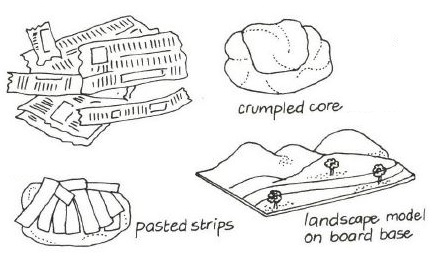
\includegraphics[width=0.45\textwidth]{./img/vso/papier-mache-layering.jpg}
\end{center}

\begin{itemize}
\item Soak small pieces, or narrow
strips, of newspaper in paste.
\item Use crumpled newspaper as a
core or skeleton for the model.
\item Build up the model in layers of
strips and pieces.
\item After drying, sandpaper smooth
and paint or varnish.
\end{itemize}


\section{Modeling Clay}

\begin{center}
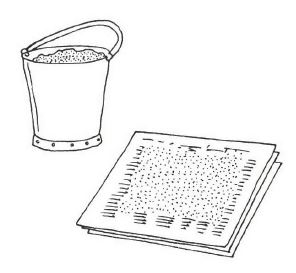
\includegraphics[width=0.4\textwidth]{./img/vso/modeling-clay.jpg}
\end{center}

\begin{itemize}
\item Dig out or collect your clay. Seek local advice on where to find
suitable deposits.
\item Add water and stir to a creamy consistency.
\item Filter through cloth or a sieve.
\item Allow the filtered material to settle.
\item Decant excess water.
\item Dry the filtered material on newspaper until it becomes a powder.
\item Mix in glycerine to give a plastic texture.
\item Knead well and add Vaseline to soften if necessary.
\item Adding paste (see page 118) to the clay helps stop it cracking as it
dries.
\end{itemize}


\section{Paste and Sand Cement} \index{Pastes}

\begin{center}
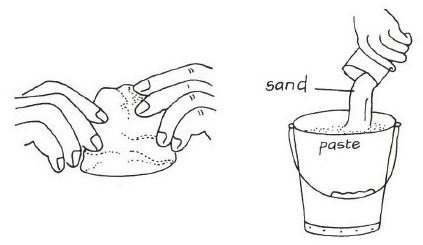
\includegraphics[width=0.4\textwidth]{./img/vso/cement.jpg}
\end{center}

\begin{itemize}
\item Mix evenly together dry sand
and flour paste
or commercial glue.
\item The wet cement moulds very
easily and dries hard.
\end{itemize}


\section{Flour Paste} %recipe? - see Flour Paste VSO 118

\begin{center}
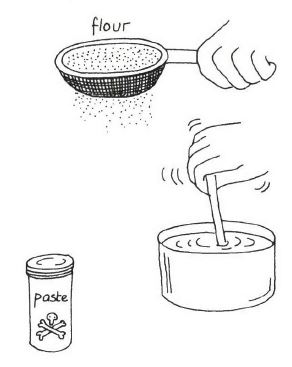
\includegraphics[width=0.4\textwidth]{./img/vso/dough.jpg}
\end{center}

\begin{itemize}
\item Sift flour to remove lumps. Maize, wheat and cassava flours are all
suitable.
\item Mix the flour with water a little at a time to avoid lumps. It should be
the consistency of thin cream.
\item Cook the mixture gently until it thickens. Keep stirring to ensure the
paste remains smooth and of even texture.
\item Allow the paste to cool.
\item Add insecticide to the paste if needed.
\item Store in a clearly labeled container with a good lid, preferably in a
cool place.
\item Cold method paste is made by simply stirring sifted flour into water.
\end{itemize}


\section{Casein Glue}

\begin{center}
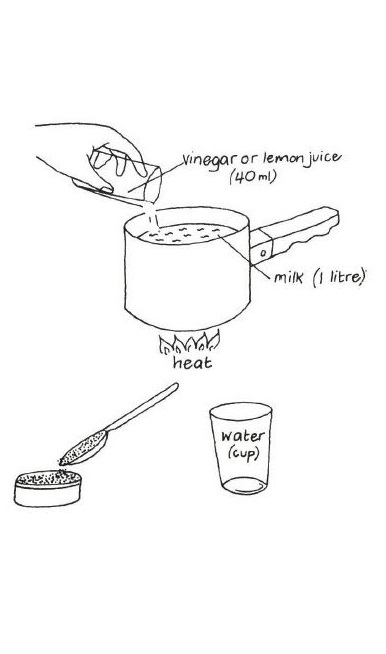
\includegraphics[width=0.4\textwidth]{./img/vso/casein-glue.jpg}
\end{center}

\begin{itemize}
\item Mix milk with vinegar or lemon
juice. Add just enough vinegar
or lemon juice to curdle the
milk. The amounts will vary
according to the type of milk
used.
\item Heat while stirring
continuously. Soft lumps will
form.
\item Strain out the lumps using a
cloth.
\item Add a teaspoon of sodium
hydrogen carbonate
(bicarbonate of soda) to the
lumps and mix with a little
water to produce casein glue.
\end{itemize}

\vfill


\end{multicols}